\subsection{\label{sec:stellarium}Stellarium}

In order to check the validity of our livestream-derived optical lightcurve, we needed a way of finding the expected eclipse obscuration percentage over time for our location.
We used the free, open-source planetarium software \texttt{Stellarium} to achieve this.
After setting the time, date and location of our radio telescope in \texttt{Stellarium}, we queried the software's API to step the simulation time forward and extracted the eclipse percentage for 1000 points in time, starting before first contact and ending after fourth contact.
The resulting theoretical lightcurve is overlaid on the eclipse obscuration derived from the UCA Observatory livestream.
The agreement between the two is excellent, validating our optical eclipse lightcurve.

\subsection{\label{sec:theoreticalLightcurves}Theoretical Lightcurve Comparison}

In order to determine the apparent radius of the sun at \unit[1420]{MHz}, we can compare our observed radio lightcurve to a theoretical lightcurve where the radius of the sun has been changed.
To accomplish this, we first downloaded high-accuracy ephemeris data from the JPL Horizons On-Line Ephemeris System. 
Using the angular radii of both the sun and moon along with the angular separation between the two, we calculated the obscured area of the solar disk at 2000 points in time during the eclipse using the geometric relationships shown in Figure \ref{fig:eclipse_geometry}.
These relationships are also given by Equations 1 through 4.

\begin{figure}
  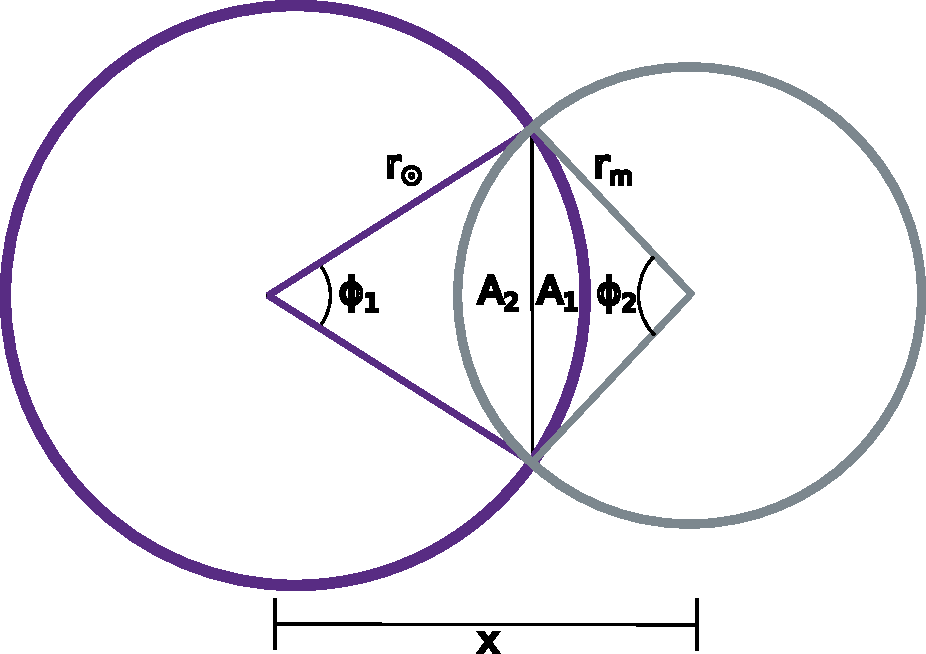
\includegraphics[width=0.5\textwidth]{figures/drawing}
  \caption{\label{fig:eclipse_geometry} The geometric relationships used to calculate the obscuration of the sun.}
\end{figure}

\begin{equation}
  A_1 = \frac{1}{2}r_{\odot}^2\left(\phi_1 - \sin\phi_1\right)
\end{equation}
\begin{equation}
  A_2 = \frac{1}{2}r_{m}^2\left(\phi_2 - \sin\phi_2\right)
\end{equation}

\begin{equation}
  \phi_1 = 2\cos^{-1}\left(\frac{r_{\odot}^2 - r_{m}^2+x^2}{2r_{\odot}x}\right)
\end{equation}
\begin{equation}
  \phi_2 = 2\cos^{-1}\left(\frac{x^2 - r_{\odot}^2 + r_{m}^2}{2r_{m}x}\right)
\end{equation}


\begin{figure}
  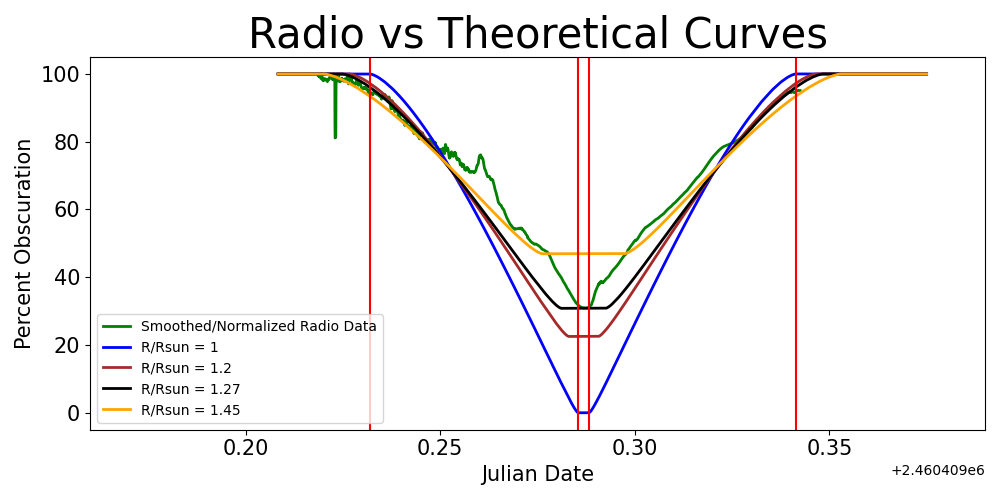
\includegraphics[width=0.5\textwidth]{figures/RadiovsTheoretical.png}
  \caption{\label{fig:RadiovsTheoretical} A comparison of the smoothed/normalized radio lightcurve and theoretical lightcurves generated with the JPL Horizons ephemeris data.}
\end{figure}

Using these relationships, we can create theoretical lightcurves for varying solar radii.
We calculated the obscured area of the solar disk at 2000 points in time during the eclipse.
Our data found that the radio lightcurve reached a minimum of 30.9\% of the total solar flux during totality, whereas the optical lightcurve reached 0\%.
Assuming a uniform disk brightness, we created theoretical lightcurves for solar radii ranging from $R = 1.0 R_{\odot}$ to $R = 1.5 R_{\odot}$.
These theoretical lightcurves, shown in Figure \ref{fig:RadiovsTheoretical}, helped us match the dip in relative difference in brightness within the radio lightcurve.
Our model does not take into acount the true non-uniformity of the solar surface, nor does it account for limb darkening.
We found that the best-fit curve has an apparent solar radius of $R_{\mathrm{1420}} = 1.27 R_{\odot}$.